\mode*
\section{Basic Building Blocks of C}

\begin{frame}[fragile]{Basic Building Blocks of C}
  \begin{iblock}{Data}
    different \alert{types} of \alert{variables}. Examples:\ttfamily
    \begin{multicols}{3}
      \begin{itemize}
      \item[int] v1;
      \item[int] v2;
      \item[int] sum;
      \item[char] c;
      \item[double] i;
      \end{itemize}
    \end{multicols}
  \end{iblock}
  \begin{iblock}{Instructions}
    Tell the computer what to do with the data.
    \begin{multicols}{2}
      \begin{itemize}
      \item Operators ($+, -, \times{}, \div{}, ...$)
      \item Assignment statement ($=$)
      \item Control statement (\mintinline{c}{if else; for; while; ...})
      \end{itemize}
    \end{multicols}
  \end{iblock}
  Examples:
  \begin{center}
\begin{ccode}
v1=5; v2=6;
sum = v1 + v2;
if (sum != 11) puts("Wrong!");
\end{ccode}    
  \end{center}
\end{frame}

\begin{frame}[fragile=singleslide]
  \begin{iblock}{Operators for shortcuts}
    \begin{center}{\ttfamily
      \begin{tabular}{llll}
        x++; & x += 2; & x *= 4; & x \%= 6;\\
        x--; & x -= 3; & x /= 5; & \\
      \end{tabular}}
    \end{center}
  \end{iblock}
\begin{ccode}
n = 5;
npp = n++; /* npp is 5 */
ppn = ++n; /* ppn is 6 */
\end{ccode}
  \begin{iblock}{The result (11 or 13) actually depends on the compiler}
    {\ttfamily
    \begin{enumerate}
    \item int i=1;
    \item i = (i++ * 5) + (i++ * 3);\quad\tikzmark{nogood}
    \end{enumerate}
    \begin{center}
      \begin{tabular}{l}
        \\
        \textcolor{red}{1}\tikzmark{a1} * 5 + \tikzmark{a2}\textcolor{red}{2} * 3 = 11\\[4ex]
        \textcolor{red}{2}\tikzmark{b2} * 5 + \tikzmark{b1}\textcolor{red}{1} * 3 = 13
      \end{tabular}
    \end{center}}
    \begin{tikzpicture}[remember picture,overlay]
      \node at (pic cs:nogood) [scale=1.2,red,opacity=.4,rotate=25] {{\humor No good}};
      \draw[overlay, ->, blue] ($(pic cs:a1)+(0,7pt)$) to [bend left=25] node [auto,inner sep=1pt] {++} ($(pic cs:a2)+(0,7pt)$);
      \draw[overlay, ->, blue] ($(pic cs:b1)+(0,7pt)$) to [bend right=25] node
      [auto,swap,inner sep=1pt] {++} ($(pic cs:b2)+(0,7pt)$);
    \end{tikzpicture}
  \end{iblock}
\end{frame}

\begin{frame}[fragile]{Functions}
    \begin{minipage}{.45\linewidth}
\begin{ccode}
int plus(int x, int y){
  int sum = x + y;
  return sum;
}
\end{ccode}      
    \end{minipage}\quad
    \begin{minipage}{.45\linewidth}
\begin{ccode}      
int main(void){
  int v1=5, v2=6;
  int sum = plus(5,6);
  return 0;
}
\end{ccode}
    \end{minipage}
    \begin{iblock}{Recursion --- A function calls itself}
      \begin{minipage}[t]{.5\linewidth}
\begin{ccode}
int factorial(int n){
  if (n == 0) return 1;
  return n*factorial(n-1);
}
\end{ccode}
      \end{minipage}\quad
      \begin{minipage}[t]{.45\linewidth}
\begin{ccode}
int main(void){
  return factorial(5);
}
\end{ccode}
      \end{minipage}
    \end{iblock}
\end{frame}

\begin{frame}{Files}{Several files can be compiled together into a single executable}
  \begin{iblock}{hello2.c}
    \begin{center}
      \mode<beamer>{ \includegraphics[width=\textwidth]{hello2-c} }%
      \mode<article>{ \cfile{../src/hello2.c}}
    \end{center}
  \end{iblock}
  \begin{center}
    \begin{minipage}[t]{.35\linewidth}
      \begin{iblock}{hello.h}
        \mode<beamer>{ 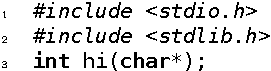
\includegraphics[width=\textwidth]{hello-h} }%
        \mode<article>{ \cfile{../src/hello.h}}
      \end{iblock}
    \end{minipage}\qquad
    \begin{minipage}[t]{.5\linewidth}
      \begin{iblock}{hi.c}
        \mode<beamer>{ 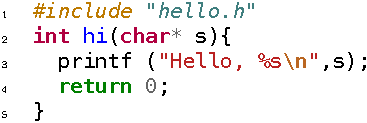
\includegraphics[width=\textwidth]{hi-c} }%
        \mode<article>{ \cfile{../src/hi.c}}
      \end{iblock}
    \end{minipage}
  \end{center}
\end{frame}

\begin{frame}{Coding Style}
\begin{center}
  \mode<beamer>{ \includegraphics[width=\textwidth]{hello-comments-c} }%
  \mode<article>{ \cfile{../src/hello-comments.c}}
\end{center}
\end{frame}

\begin{frame}{Variable Types}
  \begin{description}
  \item[Types] char, int, float, double
  \item[Qualifiers] short, long, long long, signed, unsigned
  \end{description}
  \begin{center}{\small
    \begin{tabular}{rll}\hline
      \thead{Type} & \thead{Storage size} & \thead{Value range}\\\hline
      char          & 1 byte        & ${-2^7} \sim {2^7-1}$ or $0 \sim {2^8-1}$\\
      signed char   & 1 byte        & ${-2^7} \sim {2^7-1}$\\
      unsigned char & 1 byte        & $0 \sim {2^8-1}$\\
      int           & 2 or 4 bytes  & ${-2^{15}} \sim {2^{15}-1}$ or ${-2^{31}} \sim {2^{31}-1}$\\
      unsigned int  & 2 or 4 bytes  & $0 \sim {2^{16}-1}$ or $0 \sim {2^{32}-1}$\\
      short         & 2 bytes       & ${-2^{15}} \sim {2^{15}-1}$\\
      unsigned short& 2 bytes       & $0 \sim {2^{16}-1}$\\
      long          & 4 bytes       & ${-2^{31}} \sim {2^{31}-1}$\\
      unsigned long & 4 bytes       & $0 \sim {2^{32}-1}$\\\hline
    \end{tabular}}
  \end{center}
\end{frame}

\begin{frame}{Integer}
  \begin{iblock}{Platform dependent}
    \begin{center}
      \mode<beamer>{ 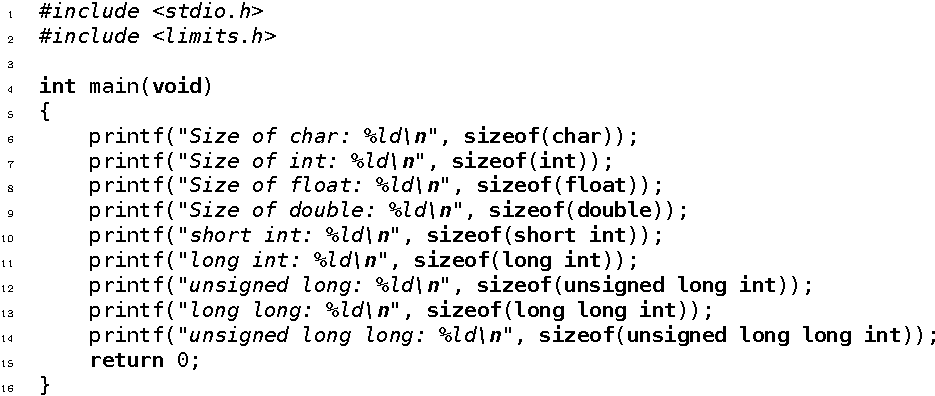
\includegraphics[width=\textwidth]{sizeof-c} }%
      \mode<article>{ \cfile{../src/sizeof.c}}
    \end{center}
  \end{iblock}
\end{frame}

See also: \citetitle[Sec 2.5, \emph{Limits}]{stevens2013advanced}.

\begin{frame}{Floating Point}
  \begin{center}{\small
    \begin{tabular}{rrlr}\hline
      \thead{Type}        &\thead{Size} &\thead{Value range}& \thead{Precision}\\\hline
float       &4 byte       &$1.2\times{}10^{-38}  \sim{}3.4\times{}10^{38}$ & 6 decimal places\\
double      &8 byte       &$2.3\times{}10^{-308} \sim{}1.7\times{}10^{308}$ & 15 decimal places\\
long double &10 byte      &$3.4\times{}10^{-4932}\sim{}1.1\times{}10^{4932}$ & 19 decimal places\\\hline
    \end{tabular}}
  \end{center}
\begin{center}
  \mode<beamer>{ 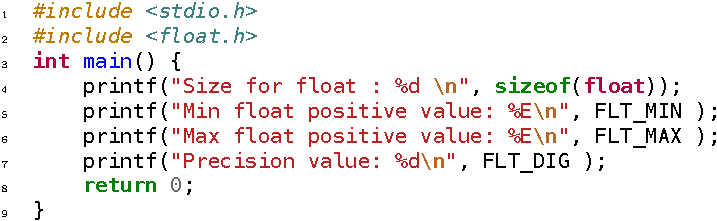
\includegraphics[width=\textwidth]{sizeoffloat-c} }%
  \mode<article>{ \cfile{../src/sizeoffloat.c}}
\end{center}
\end{frame}

\begin{itemize}
\item See also: \href{https://www.tutorialspoint.com/cprogramming/c_data_types.htm}{C data
    types}\footnote{\url{https://www.tutorialspoint.com/cprogramming/c_data_types.htm}}
\end{itemize}

\begin{frame}[fragile]{Variable Names}
  \mode<article>{\begin{multicols}{2}}
    \begin{itemize}
    \item[\Checked] \mintinline{c}{int num_of_students = 10;}
    \item[\Checked] \mintinline{c}{int numOfStudents = 10;}
    \item[\Checked] \mintinline{c}{int _numOfStudents = 10;}
    \item[\Checked] \mintinline{c}{float pi = 3.14159;}
    \item[\Checked] \mintinline{c}{int sum=0, Sum=0, SUM=0; /* case sensitive*/}
    \item[\RedCross] \mintinline{c}{3rd_entry /* starts with a number */}
    \item[\RedCross] \texttt{all\$done} \mintinline{c}{/* contains a '$'*/}%$
    \item[\RedCross] \mintinline{c}{int /* reserved word */}
    \item[\RedCross] \mintinline{c}{phone number /* has a space */}
    \end{itemize}
  \mode<article>{\end{multicols}}
  \end{frame}

\begin{frame}{Simple Operators}
\begin{center}
  \mode<beamer>{ 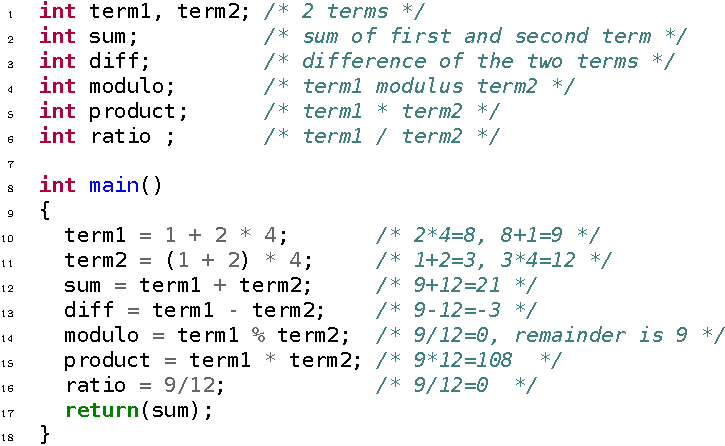
\includegraphics[width=\textwidth]{operators-c} }%
  \mode<article>{ \cfile{../src/operators.c}}
\end{center}
\end{frame}

\begin{frame}{Floating Point vs. Integer Divide}
  \begin{center}
    \begin{tabular}{lll}\hline
      \thead{Expression}&\thead{Result}&\thead{Result Type}\\\hline
      $19/10$&$1$&integer\\
      $19.0/10$&$1.9$&floating point\\
      $19.0/10.0$&$1.9$&floating point\\\hline
    \end{tabular}
  \end{center}
\end{frame}

\begin{frame}{\texttt{printf(format, expression1, expression2, ...)}}
  \begin{center}{\Large
      \mbox{{\ttfamily
          printf("\%d\tikzmark{a} times \%d\tikzmark{b} is \%d\tikzmark{c} \textbackslash n", \tikzmark{aa}2, \tikzmark{bb}3, \tikzmark{cc}2*3);}}}
  \end{center}
  \begin{tikzpicture}[remember picture,overlay, ->, opacity=.1, ultra thick]
      \draw[red] (pic cs:aa) to [bend left=15] (pic cs:a);
      \draw[blue] (pic cs:bb) to [bend left=25] (pic cs:b);
      \draw[violet] (pic cs:cc) to [bend left=35] (pic cs:c);
    \end{tikzpicture}
\end{frame}

\begin{frame}{\texttt{printf()}}{Escape Characters}
  \begin{center}
    \begin{tabular}{lll}\hline
      \thead{Character}   &\thead{Name} &\thead{Meaning}\\\hline
      \textbackslash b         &backspace       &move cursor one character to the left\\
      \textbackslash f         &form feed       &go to top of new page\\
      \textbackslash n         &newline         &go to the next line\\
      \textbackslash r         &return          &go to beginning of current line\\
      \textbackslash a         &audible alert   &‘beep’\\
      \textbackslash t         &tab             &advance to next tab stop\\
      \textbackslash ’         &apostrophe      &character ’\\
      \textbackslash "         &double quote    &character "\\
      \textbackslash\textbackslash           &backslash       &character\\
      \textbackslash nnn       &                &character number nnn (octal)\\\hline
    \end{tabular}
  \end{center}
\end{frame}

\begin{frame}{\texttt{printf()}}{Format Statements}
  \begin{center}
    \begin{tabular}{lll}\hline
      \thead{Conversion}   &\thead{Argument Type}   &\thead{Printed as}\\\hline
      \%d          &integer         &decimal number\\
      \%f          &float           &[-]m.dddddd (details below)\\
      \%X          &integer         &hex. number using A..F for 10..15\\
      \%c          &char            &single character\\
      \%s          &char *          &print characters from string until '\textbackslash 0'\\
      \%e          &float           &float in exp. form [-]m.dddddde xx\\
      ...&...&...\\\hline
    \end{tabular}
  \end{center}
  In addition,
  \begin{description}
  \item[\%6d] decimal integer, at least 6 characters wide
  \item[\%8.2f] float, at least 8 characters wide, two decimal digits
  \item[\%.10s] first 10 characters of a string
  \item[\$] \texttt{man 3 printf}
  \end{description}
\end{frame}

\begin{frame}[fragile=singleslide]{Arrays}
  \begin{iblock}{}
    \begin{center}
      \mode<beamer>{ 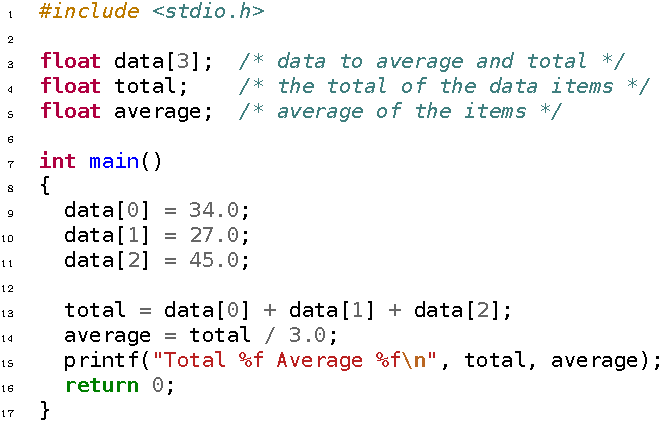
\includegraphics[width=.8\textwidth]{array1-c} }%
      \mode<article>{ \cfile{../src/array1.c}}
    \end{center}
  \end{iblock}
\begin{itemize}
\item[\Checked] \mintinline{c}{int data[3]={10,972,45};}
\item[\Checked] \mintinline{c}{int data[]={10,972,45};}
\item[\Checked] \mintinline{c}{int matrix[2][4]={{1,2,3,4},{10,20,30,40}};}
\end{itemize}
\end{frame}

\begin{frame}[fragile=singleslide]{Strings}
  \begin{description}
  \item[Strings] are \alert{character arrays} with the additional special character ``\verb|\0|''
    (NUL) at the end. E.g.:\ttfamily
    \begin{itemize}
    \item[] char system[] = "Linux";
    \item[] \begin{tabular}{*{6}{|c}|} \hline
              L&i&n&u&x&\textbackslash0\\\hline
            \end{tabular}
          \end{itemize}
  \end{description}
  \begin{iblock}{The most common string functions}
    \begin{center}
      \mode<beamer>{ 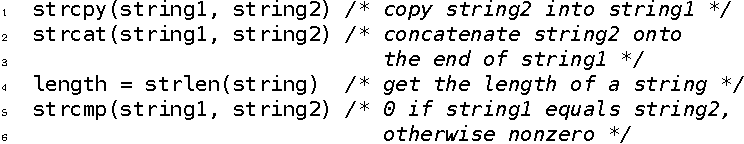
\includegraphics[width=\textwidth]{string-funcs-c} }%
      \mode<article>{ \cfile{../src/string-funcs.c}}
    \end{center}
  \end{iblock}
\end{frame}

\begin{frame}{String Functions}
  \begin{iblock}{\CMD{man 3 strcat; man 3 strcpy}}
    \mode<beamer>{ 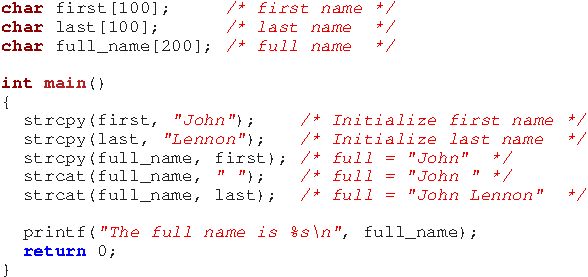
\includegraphics[width=\textwidth]{strcat-c} }%
    \mode<article>{ \cfile{../src/strcat.c}}
  \end{iblock}
\end{frame}

\begin{frame}{Reading In Strings From Keyboard}
  \begin{iblock}{\cmd{char *fgets(char *s, int size, FILE *stream);}}
    \mode<beamer>{ 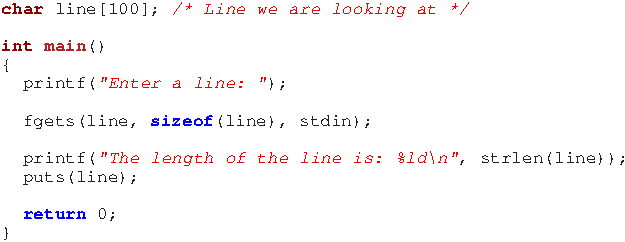
\includegraphics[width=\textwidth]{fgets1-c} }%
    \mode<article>{ \cfile{../src/fgets1.c}}
  \end{iblock}
  \begin{itemize}
  \item[\$] \texttt{man 3 fgets}
  \end{itemize}
\end{frame}

\begin{frame}
  \begin{iblock}{}
    \begin{center}
      \mode<beamer>{ \includegraphics[width=.7\textwidth]{fgets2-c} }%
      \mode<article>{ \cfile{../src/fgets2.c}}
    \end{center}
  \end{iblock}
\end{frame}

Output of fgets():
\begin{verbatim}
~$ /tmp/a.out
Enter first name: John
Enter last name: Lennon
The name is John
 Lennon
\end{verbatim}

\begin{description}
\item[What happened? Why is the last name in a new line?]  The \texttt{fgets()} function gets the
  entire line, including the end-of-line. For example, "John" gets stored as
\begin{verbatim}
{'J', 'o', 'h', 'n', '\n', '\0'}
\end{verbatim}
  This can be fixed by using the statement
\begin{verbatim}
first[strlen(first)-1] = '\0';
\end{verbatim}
  which replaces the end-of-line with an end-of-string character and so end the string
  earlier.
\end{description}

\begin{frame}{scanf()}{Reading in formatted input from stdin}
  \begin{iblock}{\cmd{int scanf(const char *format, ...);}}
    \begin{center}
      \mode<beamer>{ \includegraphics[width=.7\textwidth]{scanf-c} }%
      \mode<article>{ \cfile{../src/scanf.c} }
    \end{center}
  \end{iblock}
  \begin{itemize}
  \item Better use \texttt{fread(), fgets()} instead whenever possible
  \end{itemize}
\end{frame}

\begin{frame}{\texttt{if ... else ...}}
  \mode<beamer>{\centering\includegraphics[width=.6\textwidth]{if1-c} }%
  \mode<article>{\cfile{../src/if1.c}}
\end{frame}

\begin{frame}{Relational Operators}
  \begin{multicols}{2}
    \begin{itemize}
    \item[<] less than
    \item[<=] less than or equal
    \item[==] equal
    \item[>] greater than
    \item[>=] greater or equal than
    \item[!=] not equal
    \end{itemize}
  \end{multicols}
\end{frame}

\begin{frame}{Loops}{\texttt{while}}
  \begin{center}
    \mode<beamer>{ \includegraphics[width=.7\textwidth]{while1-c} }%
    \mode<article>{\cfile{../src/while1.c}}
  \end{center}
\end{frame}

\begin{frame}{Loops}{\texttt{for}}
  \begin{center}
    \mode<beamer>{ \includegraphics[width=.7\textwidth]{for1-c} }%
    \mode<article>{ \cfile{../src/for1.c}}
  \end{center}
\end{frame}

\begin{frame}{Loop Control Statements}{\texttt{break}}
  \begin{center}
    \mode<beamer>{ \includegraphics[width=.7\textwidth]{break-c} }%
    \mode<article>{ \cfile{../src/break.c}}
  \end{center}
\end{frame}

\begin{frame}{Loop Control Statements}{continue}
\begin{center}
  \mode<beamer>{ 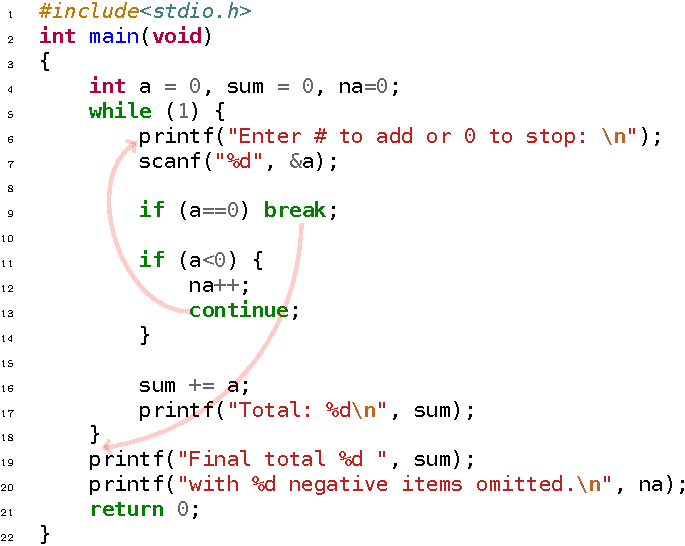
\includegraphics[width=.8\textwidth]{continue-anno} }%
  \mode<article>{ 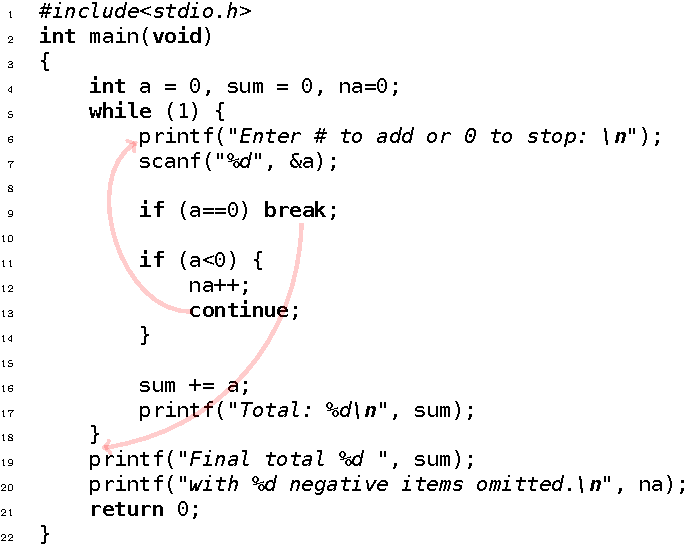
\includegraphics[width=.6\textwidth]{continue-anno-bw} }
\end{center}
\end{frame}

\begin{frame}{switch-case}
  \mode<beamer>{\centering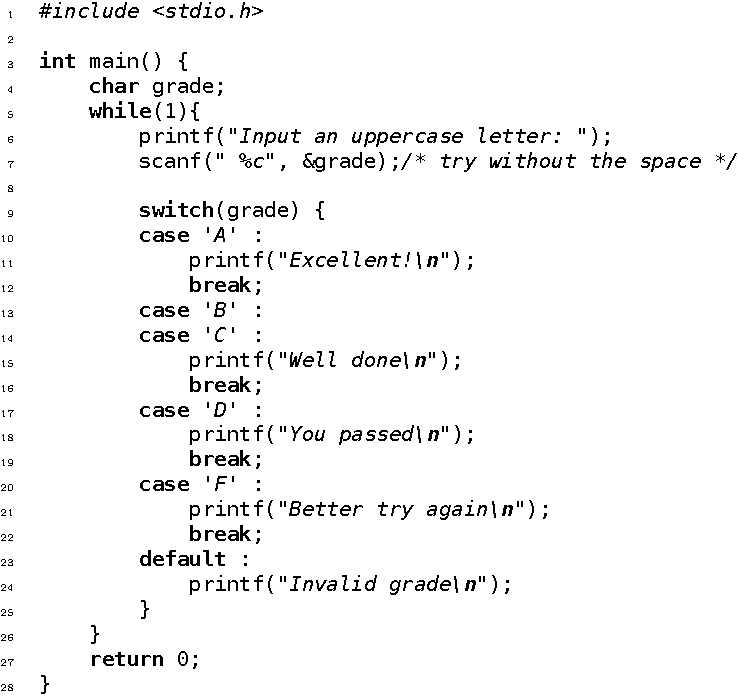
\includegraphics[width=.8\textwidth]{switch1-c} }%
  \mode<article>{\cfile{../src/switch1.c}}
\end{frame}

\begin{frame}
  \mode<beamer>{ \centering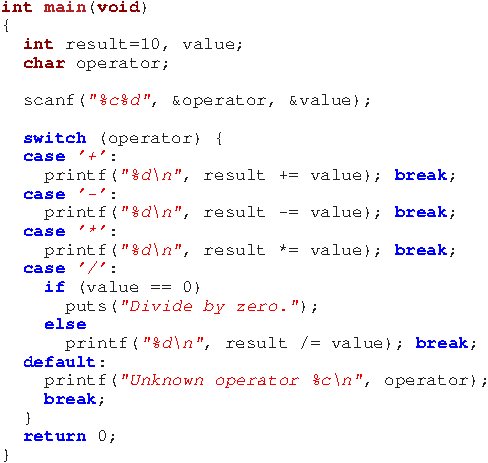
\includegraphics[width=.7\textwidth]{switch2-c} }%
  \mode<article>{ \cfile{../src/switch2.c}}
\end{frame}

\mode<all>
%%% Local Variables:
%%% mode: latex
%%% TeX-master: "c-b"
%%% End:
